\documentclass[12pt,a4paper]{article}
\usepackage[utf8]{inputenc}
\usepackage[english,czech]{babel}
\usepackage[T1]{fontenc}
\usepackage{amsmath}
\usepackage{amsfonts}
\usepackage{amssymb}
\usepackage{graphicx}
\usepackage[left=1.2cm,right=1.2cm,top=2cm,bottom=2cm]{geometry}
\usepackage[svgnames]{xcolor}
\usepackage{tabularx}
\usepackage{svg}
\usepackage{graphicx}
\usepackage{longtable}
\usepackage{booktabs}
\usepackage{fancyhdr}
\usepackage{hyperref}
\usepackage{wrapfig}
\DeclareGraphicsExtensions{.pdf,.png,.jpg}

% Redefine \includegraphics so that, unless explicit options are
% given, the image width will not exceed the width or the height of the page.
% Images get their normal width if they fit onto the page, but
% are scaled down if they would overflow the margins.
\makeatletter
\def\ScaleWidthIfNeeded{%
 \ifdim\Gin@nat@width>\linewidth
    \linewidth
  \else
    \Gin@nat@width
  \fi
}
\def\ScaleHeightIfNeeded{%
  \ifdim\Gin@nat@height>0.9\textheight
    0.9\textheight
  \else
    \Gin@nat@width
  \fi
}
\makeatother

\setkeys{Gin}{width=\ScaleWidthIfNeeded,height=\ScaleHeightIfNeeded,keepaspectratio}%


\author{ Jan Chroust }
\title{ SHT31V01A }

\fancypagestyle{all}{
  \fancyhf{}
  \fancyhead[R]{\includegraphics[height=25pt]{/home/roman/repos/MLAB/Library/Graphics/logo_MLAB_long.pdf}}
  \fancyhead[L]{ {\Huge SHT31V01A  } }
  %\fancyhead[R]{MLAB logo}
  \fancyfoot[L]{ SHT31V01A; \today; Jan Chroust; \href{http://www.mlab.cz/}{www.mlab.cz} }% Left footer
  %\fancyfoot[R]{\thepage\  / \pageref{LastPage}}% Right footer
  \fancyfoot[R]{\thepage\  of XX }% Right footer
}


\pagestyle{all}

\begin{document}
%\rmfamily
\fontsize{14.4}{20}\selectfont

\vspace*{\fill}

\begin{center}
{\Huge SHT31V1A – digitální vlhkoměr a teploměr}

{\Large Jan Chroust}

\vspace*{\fill}
\vspace*{1cm}

\end{center}
\begin{wrapfigure}{l}{4.5cm}
    
\includegraphics[width=4cm]{/home/roman/repos/newMLAB/test-mlab-repos/Modules/Sensors/SHT31V01A/DOC/SRC/img/SHT31V01A_QRcode.png}
\end{wrapfigure}

Jedná se o modul, který je možné osadit IO SHT30 nebo SHT31, které umí
měřit relativní vlhkost a teplotu s velkou přesností a stabilitou.
Rozsah měřené vlhkosti je 0 \% až 100 \%. Teplota je měřena v rozsahu
-40 C až 125 C. Komunikace probíhá přes rozhranní I2C.


\vspace*{\fill}
\vfill
\vspace*{1cm}

%% if leadImg is defined
\begin{figure}[ht!]
\centering
\includegraphics[width=10cm]{/home/roman/repos/newMLAB/test-mlab-repos/Modules/Sensors/SHT31V01A/DOC/SRC/img/SHT31V01A_top_big.jpg} 
\end{figure}
\vspace*{1cm}
%% endif

\vspace*{\fill}
\vfill
%% if Description is defined
\section{Technické parametry}\label{technickuxe9-parametry}

\begin{longtable}[c]{@{}lll@{}}
\toprule
Parametr ~ ~ ~ ~ & Hodnota ~ ~ ~ & Poznámka ~ ~ ~ ~ ~ ~\tabularnewline
\midrule
\endhead
Relativní vlhkost & 0 \% - 100 \% ~ & Typ. přesnost dle
IO\tabularnewline
Teplota ~ ~ ~ ~ ~ & -40C - 125C ~ & Typ. přesnost dle IO\tabularnewline
integrovaný obvod & SHT30, SHT31 & ~ ~ ~ ~ ~ ~ ~ ~ ~ ~\tabularnewline
Rozhraní & I2C &\tabularnewline
Napájení & Min. 2.4 V - max. 5.5 V &\tabularnewline
Rozměry & 9.65 x 40.13 mm &\tabularnewline
\bottomrule
\end{longtable}

%% endif

\flushbottom
\newpage

\section{Popis konstrukce}\label{popis-konstrukce}

\subsection{Úvodem}\label{uxfavodem}

Jedná se o modul založený na IO SHT31V01A, který umožňuje měření
relativní vlhkosti a teploty a velkou přesností a stabilitou. Další
přesné informace IO je možné vyčíst z oficiálního dokumentačního listu
výrobce. Modul obsahuje veškeré potřebné součástky pro správný chod.

\begin{figure}[htbp]
\centering
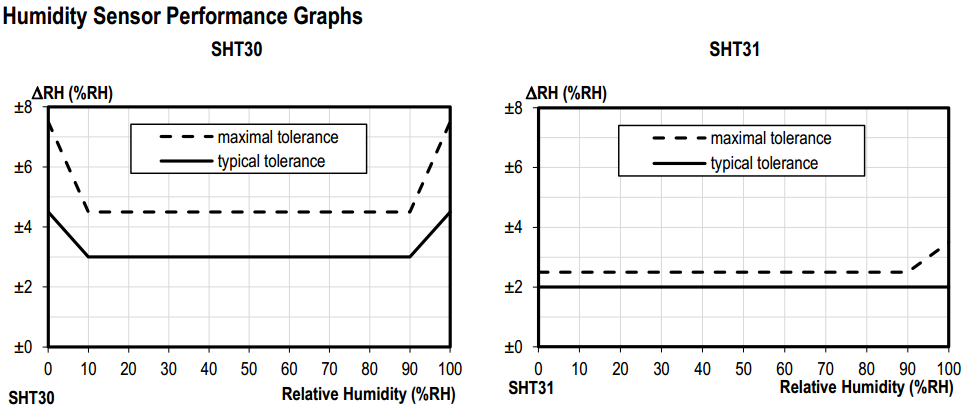
\includegraphics{DOC/SRC/img/docA.jpg}
\caption{}
\end{figure}

\begin{figure}[htbp]
\centering
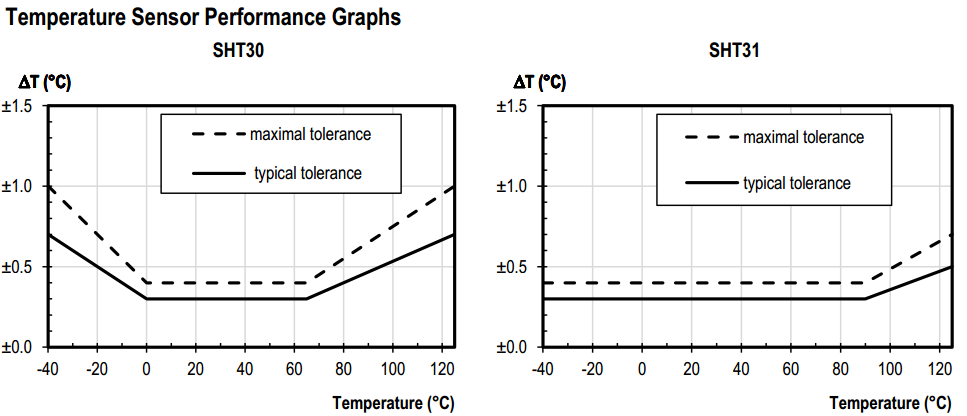
\includegraphics{DOC/SRC/img/docB.jpg}
\caption{}
\end{figure}

\newpage

\title{schema}

tady bude schema

\newpage

\section{Osazení a oživení}\label{osazenuxed-a-oux17eivenuxed}

\subsection{Osazení}\label{osazenuxed}

\begin{figure}[htbp]
\centering
\includegraphics{DOC/SRC/img/SHT31V01A_top_big.jpg}
\caption{}
\end{figure}

\subsection{Oživení}\label{oux17eivenuxed}

Je potřeba provést kontrolu zda není na plošném spoji zkrat a zda je
dobře zapájen IO. Jinak není třeba nic oživovat, pouze připojit a napsat
program. Když je nulovým odporem osazena pozice R4 adresa modulu je
0x44, pokud je osazena pozice R3 je adresa 0x45.

\subsection{Program}\label{program}

Vzorový program se nachází ve složce SW modulu. Pro spuštění je potřeba
mít nainstalovaný pyMLAB.


\end{document}